本稿では, SLSC の性質を確認するために, 真の分布から独立同分布標本を生成し, 各候補分布を当てはめた上で適合度指標を比較するモンテカルロ計算を行った.
対象分布は, Gumbel, GEV, LP3, SqrtEt, Exp, LN3 の6分布である.
各分布について, 真の分布として標本を発生させる場合と, 当てはめ分布として用いる場合の両方を考えた.

\subsection{SLSC の定義}
日本の水文頻度解析で一般に用いられてきた SLSC は, 観測値 $x_{(i)}$ を標準変量 $s=f(x)$ に写像した空間で, 観測値と理論値のずれを評価する指標である.
観測値の順序統計量に対応する標準変量を $s_{(i)}$, モデル分布に基づく理論値を $s_{(i)}^{\ast}$ とすると, SLSC は
\begin{equation}
\mathrm{SLSC}
=
\frac{
\sqrt{\dfrac{1}{N}\sum_{i=1}^{N}\bigl(s_{(i)}-s_{(i)}^{\ast}\bigr)^2}
}{
\left|s_q^{\ast}-s_{1-q}^{\ast}\right|}
\label{eq:slscs}
\end{equation}
と定義される. ここで, $q$ は上側分位を表す定数であり, 実務では $q=0.99$ が多く用いられる.
本稿では便宜的に, これを \(S\) 空間における SLSC と呼ぶ.

これに対し, 実データの空間で直接
\begin{equation}
\mathrm{SLSC}_x
=
\frac{
\sqrt{\dfrac{1}{N}\sum_{i=1}^{N}\bigl(x_{(i)}-x_{(i)}^{\ast}\bigr)^2}
}{
\left|x_q^{\ast}-x_{1-q}^{\ast}\right|}
\label{eq:slscx}
\end{equation}
と定義される量も考える.
同様に, これを \(X\) 空間における SLSC と呼ぶ.
葛葉・水木\cite{KuzuhaMizuki2022} でも指摘されているように, 標準変量が線形変換である場合には, \eqref{eq:slscs} と \eqref{eq:slscx} は一致する.
他方, 標準変量が非線形である場合には, \eqref{eq:slscs} と \eqref{eq:slscx} は一般に一致しない.
そこで本稿では, 以後 \(S\) 空間と \(X\) 空間を明示的に区別して記述し, 両者の理論的な関係は次節で整理する.

標準変量の定義は一般に一意ではなく, 代表的な定義は EVA の技術資料にも整理されている{\cite{DHI2022}}.
\rev{本稿では, \tabref{tab:standard_variate}の標準変量 $s=f(x)$ を比較用の簡易定義として用いた（GEV, LP3, SqrtEt などには形状母数を含む別定義もあり得る）.}
表の定義では, LP3 と LN3 の標準変量はいずれも元の \(x\) に対して非線形であり, それらの \(S\) 空間 SLSC は \(X\) 空間 SLSC と同一ではない.
本稿では, 非線形標準化の影響を具体的に示す代表例として, LN3 について表に示した対数標準化による \(S\) 空間評価に加えて, \(X\) 空間評価も行った.

\begin{table}[tb]
\caption{本研究で用いた標準変量 $s=f(x)$}
\label{tab:standard_variate}
\centering
\small
\setlength{\tabcolsep}{4pt}
\begin{tabular}{ll}
\hline
分布 & 標準変量 $f(x)$ \\
\hline
Gumbel & $(x-\alpha)/\beta$ \\
GEV    & $(x-\mu)/\sigma$ \\
LP3    & $\{\log x-c\}/a$ \\
SqrtEt & $bx$ \\
Exp    & $(x-c)/\mu$ \\
LN3    & $\{\log(x-c)-\mu_L\}/\sigma_L$ \\
\hline
\end{tabular}
\end{table}

\subsection{X 空間と S 空間の関係}
前節では, SLSC を \(S\) 空間と \(X\) 空間の二通りに定義した.
ここでは, 両者がどのような条件で一致し, どのような場合に異なる規準となるかを整理する.

確率紙を主たる道具としていた時代には, 確率紙上にデータをプロットし, 理論直線からのずれをその空間で評価するという発想自体は自然であった.
\figref{fig:probpaper_to_linear} は, その点を模式的に示したものである.
\figref{fig:probpaper_to_linear}(a)のように, 確率紙に相当する座標では理論関係は直線として表されるため, 標本点と理論直線の距離を測ることには手続き的な納得性がある.
しかし, 同じ関係を\figref{fig:probpaper_to_linear}(b)のように元の線形軸へ戻すと, 理論関係は一般には曲線となり, 確率紙上で同程度に見えるずれが, 元の雨量空間では異なる大きさの差に対応する.
さらに, \figref{fig:probpaper_to_linear}(c)は, この差が位置に依存する重みとして現れることを示している.
したがって, 非線形標準化を介した \(S\) 空間の SLSC は, 元の \(X\) 空間での単純な二乗平均平方根誤差ではなく, 位置依存の重みを伴う量として理解されるべきである.

\begin{figure}[tb]
  \centering
  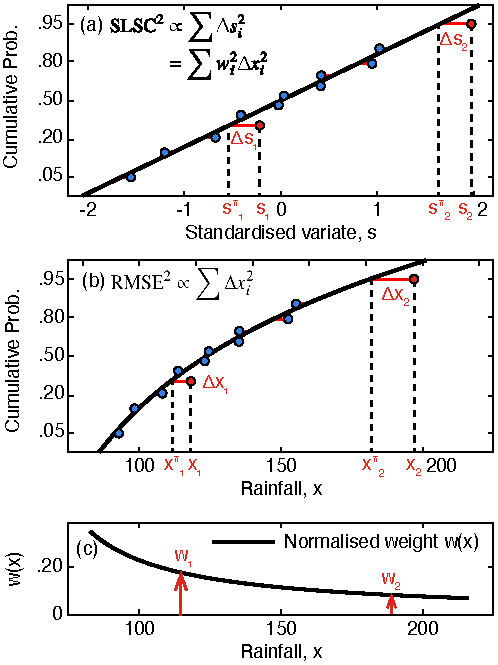
\includegraphics[width=\linewidth]{fig/method/probpaper_linear_weights_ln3_3panel_edited.pdf}
  \caption{非線形標準化における誤差評価の模式図.
  (a) 確率紙に相当する \(S\) 空間では理論関係は直線となる.
  (b) 同じ関係を雨量の \(X\) 空間へ戻すと曲線となる.
  (c) 非線形標準化では誤差評価が位置依存の重みを伴う.
  \rev{ここではシフトなしの LN3 標準化を例として示した.}}
  \label{fig:probpaper_to_linear}
\end{figure}

$f$ が $C^1$ 級関数であれば, 平均値の定理により, 各 $i$ に対して $x_{(i)}$ と $x_{(i)}^{\ast}$ の間のある点 $c_i$ が存在して,
\begin{equation}
s_{(i)}-s_{(i)}^{\ast} =
f\bigl(x_{(i)}\bigr)-f\bigl(x_{(i)}^{\ast}\bigr)
= f'(c_i)\bigl(x_{(i)}-x_{(i)}^{\ast}\bigr)
\label{eq:mvt}
\end{equation}
が成り立つ.
したがって, S 空間での二乗誤差は
\begin{equation}
\sum_{i=1}^{N}\bigl(s_{(i)}-s_{(i)}^{\ast}\bigr)^2
=
\sum_{i=1}^{N}\bigl(f'(c_i)\bigr)^2\bigl(x_{(i)}-x_{(i)}^{\ast}\bigr)^2
\label{eq:weightednorm}
\end{equation}
となる. \rev{これは X 空間での各二乗誤差に対して, 点ごとに異なる重み \(\{f'(c_i)\}^2\) を掛けた量である.}
したがって, 標準変量が線形変換であれば S 空間と X 空間の SLSC は一致するが, 非線形標準化では標準化関数に依存した距離評価となる.
より直感的に言えば, 同じ降雨量のずれであっても, 採用する分布によって大きく数えられたり小さく数えられたりすることになり, 分布ごとに異なる物差しで誤差を測っていることになる.

\subsection{ジャックナイフ法および情報量規準}
実務では, SLSCが一定の閾値を満たした候補の中からジャックナイフ幅の小さい分布を選ぶ手順が用いられることが多い{\cite{Fujibe2011}}. 本稿では, この手順を SLSC+ジャックナイフ法と呼ぶ.

ある再現期間 $T_{\mathrm{ref}}$ に対する確率水文量を $P$ とする. 標本の $i$ 番目を除いた $N-1$ 個のデータから得られる推定値を $P_i$ とすると, その平均, 標準偏差, およびジャックナイフ幅は
\begin{align}
\bar{P} &= \frac{1}{N}\sum_{i=1}^{N}P_i, \quad
s_P = \left\{\frac{1}{N}\sum_{i=1}^{N}(P_i-\bar{P})^2\right\}^{1/2}, \notag\\
W_J &= \sqrt{N-1}\,s_P
=
\left\{
\frac{N-1}{N}\sum_{i=1}^{N}\left(P_i-\bar{P}\right)^2
\right\}^{1/2}
\label{eq:jackwidth}
\end{align}
と定義される. 本稿では, 各候補分布について SLSC を計算した後, 閾値 $\mathrm{SLSC}\le 0.04$ を満たす分布の中で $W_J$ が最小となるものを採択する手順を, 実務で用いられる手順の再現として扱った.
閾値を満たす候補分布が存在しない場合には, 全候補分布の中で $W_J$ が最小となるものを採択し, その発生割合を別途確認した.
\rev{ここでの \(W_J\) は候補分布を所与とした確率水文量推定値の標本変動を表す量であり, 候補分布の真偽や推定バイアスの小ささを保証しないことに注意が必要である. 本稿では \(W_J\) 最小化を実務的手順の再現として扱う.}

比較のため, 情報量規準 AIC も算出した. AIC は $\mathrm{AIC}=-2\ell(\hat{\theta})+2k$ で定義される. ここで, $\ell(\hat{\theta})$ は最大対数尤度, $k$ は自由母数の個数である. 本稿では, Gumbel, SqrtEt, Exp を $k=2$, GEV, LP3, LN3 を $k=3$ とした.
したがって, AIC の比較には最大対数尤度の差だけでなく, 3母数分布に対して罰則項 $2k$ が1母数分大きくなる影響も含まれる.
\rev{ただし, GEV, LP3, Exp, LN3 など, 分布の定義域の端点が未知母数に依存するモデルでは, 通常の最尤推定や情報量規準の正則条件が自明ではない.
本稿では, AIC は SLSC の振る舞いを相対化するための参照として用いる.}

\subsection{数値計算の条件}
各分布について, 標本サイズを $N=25,50,\ldots,150$ とし, 真の分布から独立同分布標本を多数回発生させた.
各分布の真の母数には, 京都地点の年最大日降水量資料（1950--2024年）に各候補分布を最尤法で当てはめた推定値を用いた.
これは, 実際の水文量として現れうる尺度および歪度を反映した条件で SLSC の挙動を確認するためである.
反復数は, SLSC の標本サイズ依存性および SLSC の大きさの比較では各条件10000回とした.
一方, SLSC+ジャックナイフ法を含む採択結果の比較では計算量が大きいため, 各条件1000回とした.
このとき, ジャックナイフ幅を計算する確率水文量の参照再現期間は \(T_{\mathrm{ref}}=50\) 年とした.

各標本に対し, 候補分布ごとに母数推定を行い, X 空間の SLSC および, 必要に応じて S 空間の SLSC を算出した.
プロッティングポジションは Cunnane 式
% \begin{equation}
% p_i = \frac{i-0.4}{N+0.2}
% \label{eq:cunnane}
% \end{equation}
を用いた.
また, LN3 については, 非線形標準化の代表例として, X 空間で評価した場合と, \tabref{tab:standard_variate} に示した対数標準化で評価した場合とを分けて計算した.
これにより, 分布そのものの適合度と, 標準化の形に由来する見かけの有利性とを分離して調べることとした.
